\chapter{Design methodology and details of the calculation and device sizes of a PFD-CP Type-II $\Delta\Sigma$ Fractional-N Phase Locked Loop Simulation}
\label{ch:chap4}
\section{PLL Design Specifications}
\captionsetup{justification=centerlast} % Center the caption
\begin{center}
    \begin{table}[h]
    \centering
    \renewcommand{\arraystretch}{1.2}
    {\captionsetup{justification=centering}\caption*{\textbf{PLL Design Specifications}}}
    \begin{tabular}{l l}
        \toprule
        \textbf{Parameter} & \textbf{Project Specification} \\
        \midrule
        Technology [Min. length of transistors ($L_{min}$)] & 45 nm CMOS \\
        Supply voltage $V_{DD}$ & 1 V \\
        Nominal input common-mode voltage $V_{DD}/2$ & 0.5 V \\
        \midrule
        Reference frequency $f_{REF}$ & 200 MHz \\
        Fractional division ratio $N$ & $2 \leq N \leq 16$ \\
        Output frequency range $f_{OUT}$ & $f_{OUT,min}$ GHz -- $f_{OUT,max}$ GHz \\
        PLL lock time $t_{lock}$ & $t_{lock,min}$ ps -- $t_{lock,max}$ ps \\
        Overall average DC power consumption $P_{total,avg}$ & ? $\mu$W \\
        \bottomrule
    \end{tabular}
    \end{table}
\end{center}


\section{A type I CC LC voltage-controlled oscillator (VCO) with MOS varactors}
\begin{figure}[h]
    \centering
    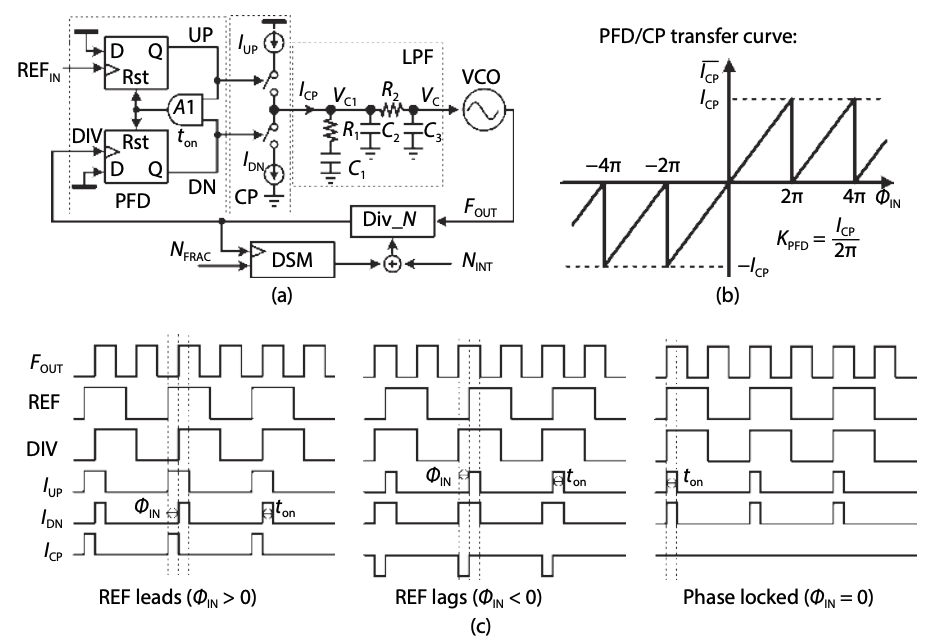
\includegraphics[width=0.9\textwidth]{images/A3-1.png}
    \caption{A PFD-CP Type-II $\Delta\Sigma$ Fractional-N Phase Locked Loop Simulation}
\end{figure}



\section{Pre-Calculations}

\section*{Design Methodology and Device Sizes}

The design of a Type-II $\Delta\Sigma$ Fractional-N Phase-Locked Loop (PLL) in 45\,nm CMOS involves several key steps, incorporating analog and mixed-signal blocks. Here's a structured methodology tailored to this project:

\subsection*{1. Architecture Selection}
\begin{itemize}
    \item Start with the block architecture shown in Figure~1(a).
    \item Replace the LC-VCO with a \textbf{Ring VCO} for better integration and wider tuning range.
    \item Use a \textbf{4-bit binary counter (MOD-16)} instead of DSM for simplicity.(Not used)
\end{itemize}

\subsection*{2. Block-Level Design}
\begin{itemize}
    \item \textbf{Phase Frequency Detector (PFD)}:
    \begin{itemize}
        \item Tri-state PFD with reset to reduce dead zone.
        \item Key parameters: propagation delay and dead zone minimization.
    \end{itemize}
\section*{PFD Functionality Explanation}

This PFD has:

\subsection*{Inputs:}
\begin{itemize}
    \item \textbf{REF} — the reference clock input
    \item \textbf{DIV} — the feedback clock input (from divider output)
\end{itemize}

\subsection*{Outputs:}
\begin{itemize}
    \item \textbf{UP}, \textbf{DN} — these are the charge pump control signals.
\end{itemize}

\subsection*{Working:}
\begin{itemize}
    \item If REF edge arrives before DIV, the PFD generates a high UP pulse.
    \item If DIV edge arrives before REF, the PFD generates a high DN pulse.
    \item If they arrive simultaneously, no output pulse is generated (ideal lock condition).
\end{itemize}

\subsection*{Internal Blocks:}
\begin{itemize}
    \item Two D flip-flops (made using NAND and NOT gates) — one for REF, one for DIV.
    \item One Reset Logic (AND gates) to detect when both outputs (UP and DN) are high and reset both flip-flops.
\end{itemize}

Thus,
\[
\text{UP pulse width} \propto \text{phase difference (REF leads DIV)}
\]
\[
\text{DN pulse width} \propto \text{phase difference (DIV leads REF)}
\]

This tri-state behavior ensures minimal dead zone and fast locking.

\section*{2. Device Sizing for 45\,nm CMOS}

Since the technology is 45\,nm, and this circuit operates at high frequencies (up to $\sim$3.2\,GHz), we require fast gates.

\subsection*{Typical Sizing:}

\begin{center}
\
\begin{tabular}{|>{\raggedright\arraybackslash}p{5cm}|>{\raggedright\arraybackslash}p{8cm}|}
\hline
\textbf{Block} & \textbf{Devices} \\ \hline
Inverter (inside flip-flop and output drivers) & NMOS: $2\,\mu m/45\,nm$ \newline PMOS: $4\,\mu m/45\,nm$ \\ \hline
NAND gate & NMOS (each): $1.5\,\mu m/45\,nm$ \newline PMOS (each): $3\,\mu m/45\,nm$ \\ \hline
AND gate (reset logic) & NMOS (each): $1.5\,\mu m/45\,nm$ \newline PMOS (each): $3\,\mu m/45\,nm$ \\ \hline
Buffer stages (driving UP/DN) & NMOS: $2.5\,\mu m/45\,nm$ \newline PMOS: $5\,\mu m/45\,nm$ \\ \hline
\end{tabular}
\end{center}

All transistors use minimum length $L=45\,\text{nm}$.

\textbf{Note:} PMOS are wider than NMOS because PMOS mobility is about 2–3x lower than NMOS.

Buffers on UP/DN signals are slightly upsized to drive the charge pump inputs fast and sharply.

\section*{3. Important Calculations}

\subsection*{3.1 Dead Zone Time}

The dead zone arises due to internal mismatch and delays.

Dead zone time ($t_{\text{DZ}}$) is minimized by:
\begin{itemize}
    \item Matching the delay paths
    \item Making reset gates faster
\end{itemize}

Typically targeted $t_{\text{DZ}} < 5\,\text{ps}$.

\subsection*{3.2 Maximum Frequency}

Since the target is $f_{\text{REF}} = 200\,\text{MHz}$ and VCO up to 3.2\,GHz, the PFD must work reliably up to 3.2\,GHz.

Thus, the PFD maximum operating frequency $f_{\text{max}}$:

\[
f_{\text{max}} \approx \frac{1}{2t_{\text{setup}}}
\]
where $t_{\text{setup}}$ is the setup time of flip-flop plus reset delay.

Typically:
\[
t_{\text{setup}} + t_{\text{reset}} \sim 50\,\text{ps}
\]

Thus:
\[
f_{\text{max}} \approx 10\,\text{GHz}
\]
which is comfortably safe.

\subsection*{3.3 Power Estimation}

Dynamic Power of PFD:

\[
P = \alpha C_{\text{load}} V_{\text{DD}}^2 f
\]
where:
\begin{itemize}
    \item $\alpha \approx 1$ (for toggle-heavy signals)
    \item $C_{\text{load}} \approx 10\,\text{fF}$ per gate
    \item $V_{\text{DD}} = 1\,\text{V}$
    \item $f = 200\,\text{MHz}$ to $3.2\,\text{GHz}$
\end{itemize}

Example at 3.2\,GHz:

\[
P_{\text{gate}} \approx 10\,\text{fF} \times (1)^2 \times 3.2\,\text{GHz} = 32\,\mu\text{W} \quad (\text{per gate})
\]

For the whole PFD ($\sim$20 gates), total:

\[
P_{\text{PFD}} \approx 0.6\,\text{mW}
\]

    \item \textbf{Charge Pump (CP)}:
    \begin{itemize}
        \item Matched current sources/sinks to ensure linearity.
        \item Target current mismatch $<$ 1\% for better phase noise performance.
    \end{itemize}

    \item \textbf{Loop Filter (LPF)}:
    \begin{itemize}
        \item Design a second-order passive filter.
        \item Select component values to balance loop bandwidth and stability:
        \[
        R_1 = 10\,k\Omega,\quad C_1 = 10\,pF,\quad C_2 = 1\,pF
        \]
    \end{itemize}
\section{Functionality Explanation}
This circuit is a high-swing NMOS-switched charge pump. It is designed to:
\begin{itemize}
    \item Provide matched UP and DOWN currents.
    \item Increase output voltage swing (even close to VDD and GND).
    \item Reduce mismatch between sourcing and sinking currents (important for low jitter and low spurs).
\end{itemize}

\subsection*{Key Blocks}
\begin{itemize}
    \item \textbf{Current Source}: A bias current source ($I_{CP} = 80\,\mu A$) supplies a constant current.
    \item \textbf{PMOS Current Mirrors (MP1--MP5)}: Mirror and split the bias current to the upper branch.
    \item \textbf{NMOS Current Mirror (MN1--MN3)}: Mirror the current for the sinking (down) branch.
    \item \textbf{Switching Transistors (MN5, MN6, MN7, MN8)}: Turned ON/OFF by the PFD outputs (UPB, DN, DN, DNB).
    \item \textbf{High-Swing Cascode Structure}: MP2 and MP3 (for sourcing) and MN2 and MN3 (for sinking) form cascoded current sources to increase output resistance, improving matching.
    \item \textbf{Output Node ($V_{\text{cnt}}$)}: Net result of charging or discharging depending on PFD control.
\end{itemize}

\section{Transistor Device Sizes}
\begin{center}
\begin{tabular}{|c|c|}
\hline
\textbf{Transistor} & \textbf{W/L ($\mu$m/$\mu$m)} \\ \hline
MP0 & 40/5 \\ \hline
MP1 & 40/5 \\ \hline
MP2 & 110/2 \\ \hline
MP3 & 110/2 \\ \hline
MP4 & 5/0.5 \\ \hline
MP5 & 5/0.5 \\ \hline
MN1 & 20/2 \\ \hline
MN2 & 20/2 \\ \hline
MN3 & 20/2 \\ \hline
MN5 & 20/2 \\ \hline
MN6 & 20/2 \\ \hline
MN7 & 100/2 \\ \hline
MN8 & 100/2 \\ \hline
\end{tabular}
\end{center}

\textbf{Notes:}
\begin{itemize}
    \item PMOS devices are generally wider to compensate for lower hole mobility.
    \item Cascode devices (MP2, MP3, MN2, MN3) are wider to ensure minimal voltage drop and maintain high output impedance.
    \item Switches MN7, MN8 are very wide (100 $\mu$m) to minimize voltage drop and resistive loss when turned ON.
\end{itemize}

\section{Important Calculations}

\subsection{Matching Error}
Mismatch causes phase noise and spurs. The mismatch $\delta$ between sourcing and sinking currents should be:
\[
\delta = \frac{|I_{up} - I_{down}|}{I_{cp}} \leq 1\%
\]
where $I_{cp} = 80\,\mu A$.

Thus:
\[
|I_{up} - I_{down}| \leq 0.8\,\mu A
\]

\subsection{Output Voltage Range}
Thanks to the high-swing cascodes, the output ($V_{\text{cnt}}$) swing is improved:

\[
V_{out,\text{max}} \approx V_{DD} - V_{SG} - V_{DS,\text{sat}}
\]
\[
V_{out,\text{min}} \approx V_{DS,\text{sat}}
\]

Given:
\begin{itemize}
    \item $V_{SG} \approx 0.25\,V$
    \item $V_{DS,\text{sat}} \approx 0.1\,V$
\end{itemize}

Thus:
\[
V_{out,\text{max}} \approx 1\,V - 0.25\,V - 0.1\,V = 0.65\,V
\]
\[
V_{out,\text{min}} \approx 0.1\,V
\]

This is sufficient because the VCO control voltage typically varies between $0.1\,V$ and $0.9\,V$.

\subsection{Charge Pump Gain}
The charge pump gain $K_{CP}$ is:

\[
K_{CP} = \frac{I_{cp}}{2\pi}
\]

Given $I_{cp} = 80\,\mu A$:

\[
K_{CP} = \frac{80 \times 10^{-6}}{2\pi} \approx 12.7\,\mu A/\text{rad}
\]

This value is used in the PLL open-loop gain calculation.

\section{Final Summary}

\begin{center}
\begin{tabular}{|l|l|}
\hline
\textbf{Item} & \textbf{Value} \\ \hline
Technology & 45 nm CMOS \\ \hline
$V_{DD}$ & 1 V \\ \hline
$I_{CP}$ & 80 $\mu$A \\ \hline
PMOS Sizes & MP0, MP1: 40/5; MP2, MP3: 110/2; MP4, MP5: 5/0.5 \\ \hline
NMOS Sizes & MN1--MN3: 20/2; MN5, MN6: 20/2; MN7, MN8: 100/2 \\ \hline
Matching Error & $<1\%$ \\ \hline
Output Voltage Range & $\sim 0.1V$ to $0.65V$ \\ \hline
$K_{CP}$ & $\sim 12.7\,\mu A/\text{rad}$ \\ \hline
\end{tabular}
\end{center}



    \item \textbf{Ring VCO}:
    \begin{itemize}
        \item Implement a 3-stage or 5-stage differential ring oscillator.
        \item Use tail current source for linear tuning.
        \item Frequency tuning range should cover 2\,GHz to 3.2\,GHz (based on $N = 2$ to $16$ with $f_{\text{REF}} = 200$\,MHz).
    \end{itemize}

\section{Functionality of the Ring VCO}

The Ring VCO consists of an odd number (here, 5) of inverter stages connected in a ring (feedback from last output to the first input).

\begin{itemize}
    \item Each inverter introduces a delay, and the total delay around the ring determines the oscillation frequency.
    \item The delay --- and thus the frequency --- is controlled using a control voltage ($V_{ctrl}$).
    \item NMOS and PMOS transistors are used as current sources controlled by $V_{ctrl}$ (common in current-starved inverters).
\end{itemize}

\section{Basic Working Principle}

\begin{itemize}
    \item Inverter delay is proportional to the supply current.
    \item $V_{ctrl}$ changes the current through each inverter stage.
    \item Higher $V_{ctrl} \rightarrow$ higher current $\rightarrow$ faster switching $\rightarrow$ higher frequency.
    \item Lower $V_{ctrl} \rightarrow$ lower current $\rightarrow$ slower switching $\rightarrow$ lower frequency.
\end{itemize}

The oscillation frequency $f_{osc}$ is approximately:

\[
f_{osc} = \frac{1}{2N t_d}
\]

where:
\begin{itemize}
    \item $N$ = number of stages (here, 5),
    \item $t_d$ = delay per inverter stage.
\end{itemize}

\section{Device Sizing (General Guide)}

To design properly, a balance must be struck between:
\begin{itemize}
    \item Speed (lower delay),
    \item Power consumption (lower current),
    \item Swing (rail-to-rail output if needed).
\end{itemize}

Typical initial sizing approach:

\begin{itemize}
    \item Use an NMOS and PMOS pair per inverter.
    \item Assume minimum channel length for the technology (e.g., $L = 45\,\mathrm{nm}$).
\end{itemize}

Widths:
\begin{itemize}
    \item NMOS width $W_n$: 2–5$\times$ minimum width,
    \item PMOS width $W_p$: $1.5\times W_n$ to $2\times W_n$ (to compensate for lower hole mobility).
\end{itemize}

Example sizing (for 45nm technology):

\[
L = 45\,\mathrm{nm}
\]
\[
W_n = 200\,\mathrm{nm}, \quad W_p = 300\,\mathrm{nm}
\]

Later adjustment is needed based on simulation results (targeting desired $f_{osc}$, power, tuning range, etc.).

\section{Key Calculations}

Suppose the target is:

\[
f_{osc} = 1\,\mathrm{GHz}
\]

Then the delay per stage needed:

\[
t_d = \frac{1}{2Nf_{osc}} = \frac{1}{2\times5\times1\times10^9} = 100\,\mathrm{ps}
\]

Thus, each inverter must have a delay of approximately 100 ps.

Controlling:

\begin{itemize}
    \item Drive current $I_d$ of NMOS/PMOS,
    \item Load capacitance $C_L$ per stage.
\end{itemize}

Approximate relation:

\[
t_d \approx \frac{C_L V_{DD}}{I_d}
\]

where:
\begin{itemize}
    \item $C_L$ includes parasitic capacitance (input capacitance of next stage + wiring),
    \item $I_d$ depends on sizing and overdrive voltage.
\end{itemize}

Adjust $W/L$ to control current.

\section{Extra Design Notes}

\begin{itemize}
    \item The number of stages must be odd (for oscillation).
    \item $V_{ctrl}$ often biases a current source that sets inverter strength.
    \item Add an output buffer if the VCO output needs to drive large loads.
\end{itemize}

Simulation: After schematic, simulate VCO's $f_{osc}$ vs $V_{ctrl}$ curve (known as the VCO Gain, $K_{VCO}$):

\[
K_{VCO} = \frac{d f_{osc}}{d V_{ctrl}} \quad [\mathrm{Hz/V}]
\]

\section{Summary of Needed Parameters}

\begin{center}
\begin{tabular}{|c|c|}
\hline
\textbf{Parameter} & \textbf{Suggested Initial Value} \\
\hline
Technology & 45nm CMOS \\
\hline
NMOS Width $W_n$ & 200 nm \\
\hline
PMOS Width $W_p$ & 300–400 nm \\
\hline
Channel Length $L$ & 45 nm \\
\hline
Supply Voltage $V_{DD}$ & 1V (check your tech file) \\
\hline
Target Frequency $f_{osc}$ & 500 MHz – 2 GHz \\
\hline
Number of Stages $N$ & 5 \\
\hline
\end{tabular}
\end{center}


    \item \textbf{Frequency Divider}:
    \begin{itemize}
        \item Synchronous 4-bit binary counter using D flip-flops.
        \item Designed to handle VCO frequencies up to 3.2\,GHz.
    \end{itemize}
\end{itemize}

\subsection*{3. Loop Parameter Calculation}
Use the classical linear PLL model for the open-loop transfer function:
\[
H(s) = \frac{K_{\text{PD}} \cdot I_{\text{CP}} \cdot Z(s) \cdot K_{\text{VCO}}}{s}
\]

Where:
\[
K_{\text{PD}} = \frac{I_{\text{CP}}}{2\pi}, \quad Z(s) \text{: Transfer function of the loop filter}, \quad K_{\text{VCO}} \text{: VCO gain in rad/V$\cdot$s}
\]

Design targets:
\begin{itemize}
    \item Loop bandwidth $\approx \frac{1}{10} f_{\text{REF}}$ (i.e., 20\,MHz)
    \item Phase margin $\geq 60^\circ$
    \item Lock time $<$ 1\,$\mu$s
\end{itemize}

\subsection*{4. Device Sizing}
Use minimal length $L = 45$\,nm throughout.

\begin{itemize}
    \item \textbf{PFD}:
    \begin{itemize}
        \item Inverter transistors: $W/L = 2\,\mu\text{m} / 45\,\text{nm}$
        \item NAND gates: $W/L = 1.5\,\mu\text{m} / 45\,\text{nm}$
    \end{itemize}

    \item \textbf{Charge Pump}:
    \begin{itemize}
        \item Current mirror: PMOS \& NMOS: $W/L = 3\,\mu\text{m} / 45\,\text{nm}$
        \item Switching transistors: $W/L = 1\,\mu\text{m} / 45\,\text{nm}$
    \end{itemize}

    \item \textbf{VCO}:
    \begin{itemize}
        \item Differential pair: $W/L = 5\,\mu\text{m} / 45\,\text{nm}$
        \item Tail current source: $W/L = 4\,\mu\text{m} / 45\,\text{nm}$
        \item Output load devices: $W/L = 2\,\mu\text{m} / 45\,\text{nm}$
    \end{itemize}

    \item \textbf{Divider Flip-Flops}:
    \begin{itemize}
        \item Inverter/clocked transistors: $W/L = 1\,\mu\text{m} / 45\,\text{nm}$
    \end{itemize}

    \item \textbf{Biasing circuits}:
    \begin{itemize}
        \item Typically: $W/L = 5\,\mu\text{m} / 45\,\text{nm}$
    \end{itemize}
\end{itemize}

\subsection{Transistor Parameters from Cadence Simulation}

\section{Details of the Calculation and Device Sizes}



\section{Summary of Calculated Values}

\begin{table}[h]
    \centering
        {\captionsetup{justification=centering}\caption*{\textbf{Summary of Calculated Values} }}
    \renewcommand{\arraystretch}{1.2} % Adjust row spacing
    \begin{tabular}{lcccc} % Removed vertical bars for cleaner look
        \toprule
        \textbf{Parameter}& \textbf{Approximated} & \textbf{Chosen} & \textbf{Unit} \\
        \midrule
        Length of $M_{1,2}$& 1& 1 & $\mu$m \\
        Width of $M_{1,2}$ & 5 & 5 & $\mu$m \\
        Length of $M_{3,4}$& 1& 1 & $\mu$m \\
        Width of $M_{3,4}$ & 10 & 10 & $\mu$m \\
        Length of varators $M_{v1,v2}$& 1 & 10& $\mu$m \\
        Width of varators $M_{v1,v2}$ & 5 & 10 & $\mu$m \\
        Inductance $L_{1}$ & 10 & 5 & $\nano$H\\
        Bias current $I_{bias}$ & 200 & 800 & $\mu$A \\  
        Control voltage $V_{cont}$ & - & 320 & $\milli$V \\   
        \bottomrule
    \end{tabular}
    \label{tab:summary_values}
\end{table}

\begin{table}[h]
    \centering
    \captionsetup{justification=centering} % Ensure centering
    \caption*{\textbf{Summary of Calculated Values of Transistors}} % Centered caption
    \renewcommand{\arraystretch}{1.2} % Adjust row spacing
    \begin{tabular}{lccc} % Ensuring correct column alignment
        \toprule
        \textbf{Transistor} & \textbf{Length} & \textbf{Width} & \textbf{Unit} \\
        \midrule
        $M_1$ & 1 & 5 & $\mu$m  \\
        $M_2$ & 1 & 5 & $\mu$m \\
        $M_3$ & 1 & 10 & $\mu$m  \\
        $M_4$ & 1 & 10 & $\mu$m  \\
        $M_{V1}$ & 1 & 5 & $\mu$m  \\
        $M_{V2}$ & 1 & 5 & $\mu$m \\
        \bottomrule
    \end{tabular}
    \label{tab:summary_values} % Table label should come after the tabular environment
\end{table}



\endinput